\documentclass[12pt]{article}

% Packages

% for floating graphics w/ captions
\usepackage{graphicx}
\usepackage{caption}
\usepackage{subcaption}
\usepackage{float}

% for math stuffs
\usepackage{amsmath}

% for math notes
\usepackage[hide]{ed}

\title{Kuramoto Oscillator}
\author{Tom Wiesing \\ Alee Kazmi}
\date{\today}

\begin{document}
	
	% Title Page
	\maketitle
	\newpage
	
	% Table of content
	\tableofcontents
	% TODO: Insert who wrote which section
	\newpage
	
	% Section 1
	\section{Introduction}
	\label{sec:intro}

\subsection{Oscillators}
Oscillators can be described as a repetitive motion of some measure about a central value which is often the point of equilibrium. This term is often used in mechanical systems but it must also be noted that oscillations occur in dynamic systems too, such as economic graphs, geothermal temperatures across areas and periodic ``firing'' of fireflies in nature. Some examples of oscilating objects can be found in Figure~\ref{fig:intro_samples}. 

\begin{figure}[h]
\centering
\begin{subfigure}{.4\textwidth}
  \centering
  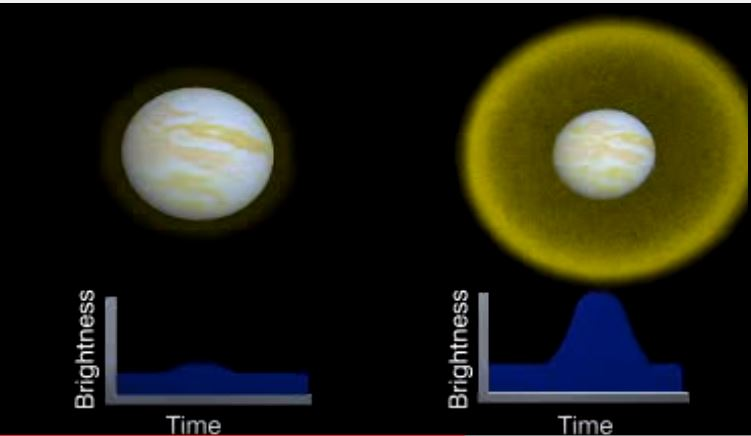
\includegraphics[width=\textwidth]{imgs/cepheid}
  \caption{Cepheid Stars that are known to flash occasionally. Such a flash is an example of an oscilation. }
\end{subfigure}%
\space\space\space
\begin{subfigure}{.5\textwidth}
  \centering
  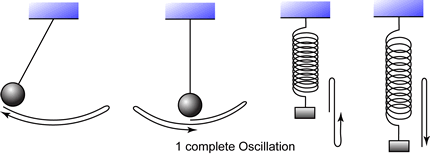
\includegraphics[width=\textwidth]{imgs/oscillation}
  \caption{An pendulum swinging to the left and right and a spring oscilating up and down. }
\end{subfigure}
\caption{Some examples of oscilating objects}
\label{fig:intro_samples}
\end{figure}


\subsection{Coupling}
Coupled Oscillation are a slightly more complex form of ordinary oscillators. In this model the oscillators are connected such that energy can be transferred between them. This motion can be very complex and does not have to be periodic. However, in the bigger scheme of things, every oscillator can be viewed as having a very well defined frequency of its own. Perhaps the simplest example of coupling could is a gear that transmits torque between two shafts (see Figure~\ref{fig:intro_gear}) that are not collinear. 

\begin{figure}[h]
  \centering
  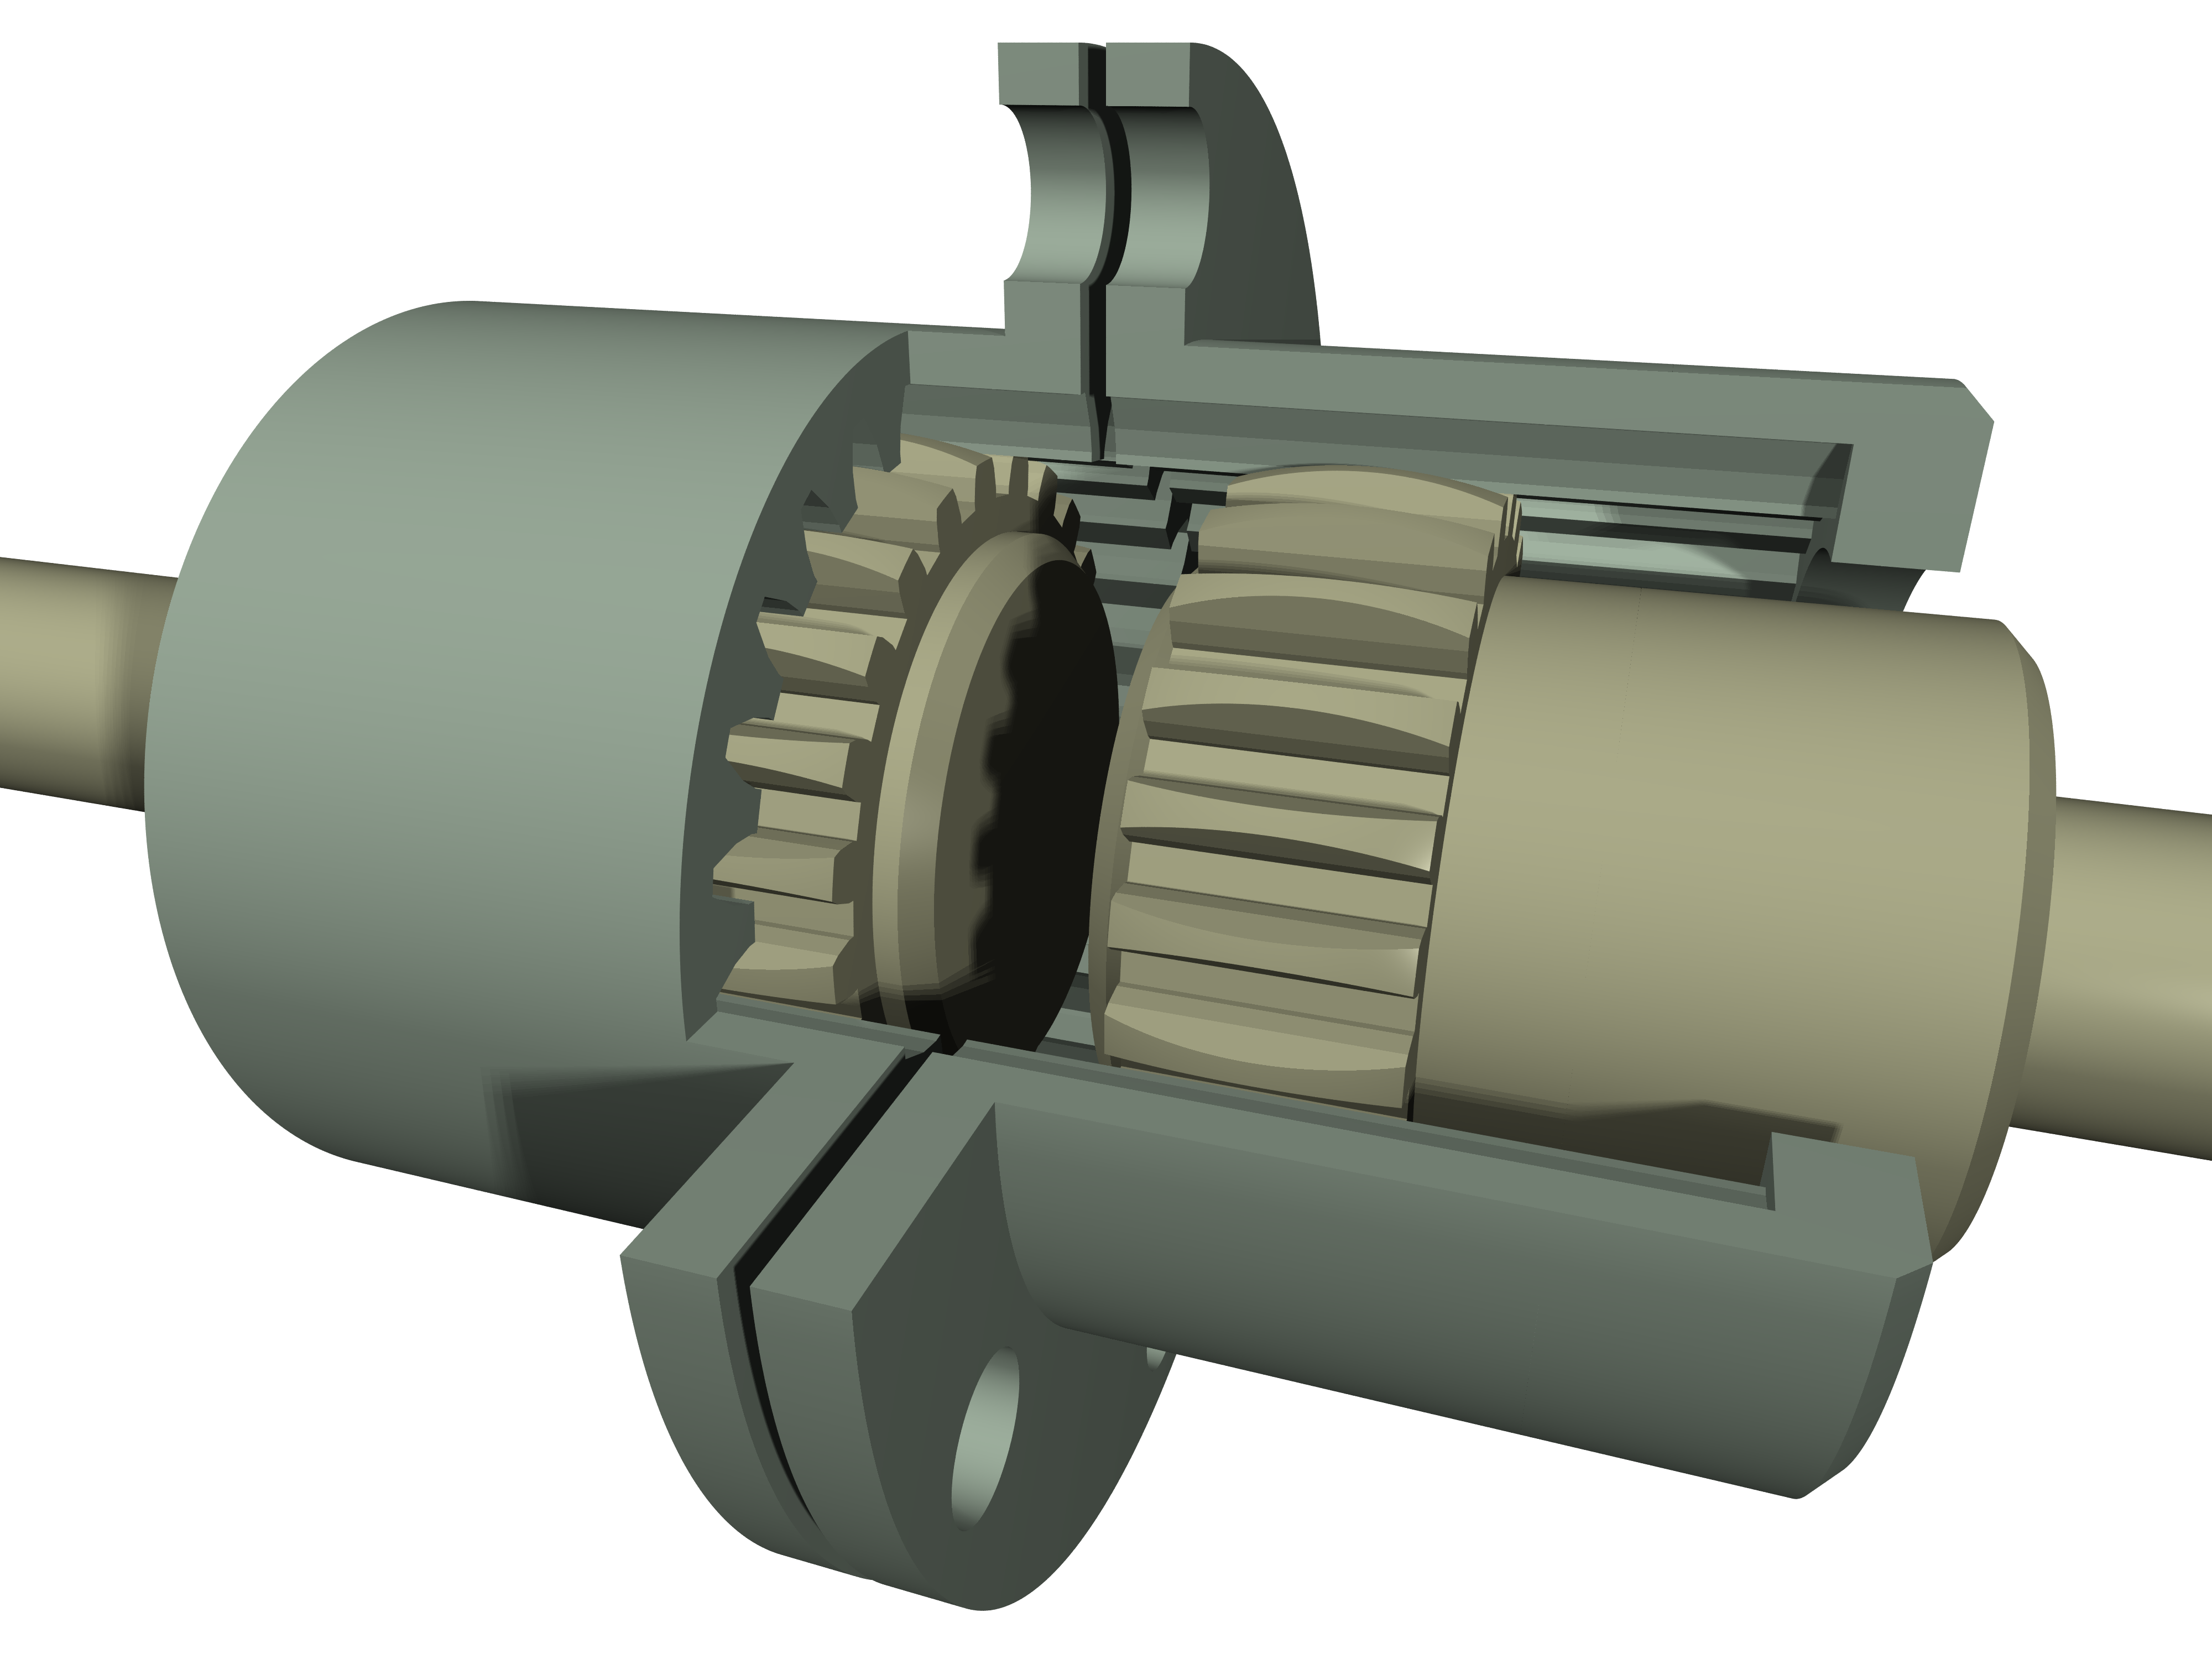
\includegraphics[width=.5\textwidth]{imgs/gear}
  \caption{Image of a gear that transmits torque beween two non-collinear shafts. }
  \label{fig:intro_gear}
\end{figure}

A slightly more complex situation arises when two pendulums are joined together by an energy medium, for example a string. As we can see in Figure~\ref{fig:intro_couple}, the two pendula have opposite amplitudes: The first pendulum only attains its maximum amplitude when the second has its lowest one. This form of synchronization behaviour can only be achieved after sufficient time has passed. 

\begin{figure}[h]
\centering
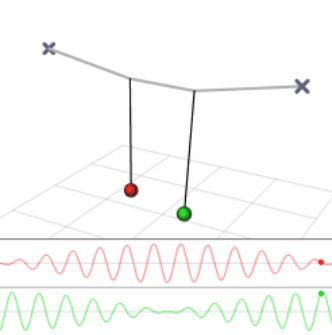
\includegraphics[width=.5\textwidth]{imgs/couple}
\caption{Two oscilating springs that exhibit coupling behaviour because they are connected through a string}
\label{fig:intro_couple}
\end{figure}

\subsection{Attaining Synchronisation}

In any oscilating system of multiple objects synchronization can occur in two ways, (1) through coupling or (2) through randomness. In the first case some form of communication between the oscilators occurs allowing them to couple. In the second case it just so happens that they start out in a similar situation and are naturally synchronized. In this study we are only interested in the first case. 

Communication can be achieved by using a medium such as a string between oscilators or by just the intrinsic tendency of natural beings to produce a unison of movement, such as fireflies flashing or humans clapping in a room. 

\subsection{The Firefly model}

The firefly flashing, more commonly known as the firefly model, is a classic example of synchronisation. This is modelled in detail by Kuramoto oscilators which is the main topic of study for this report. We will introduce these in the next section. 

\begin{figure}[h]
	\centering
	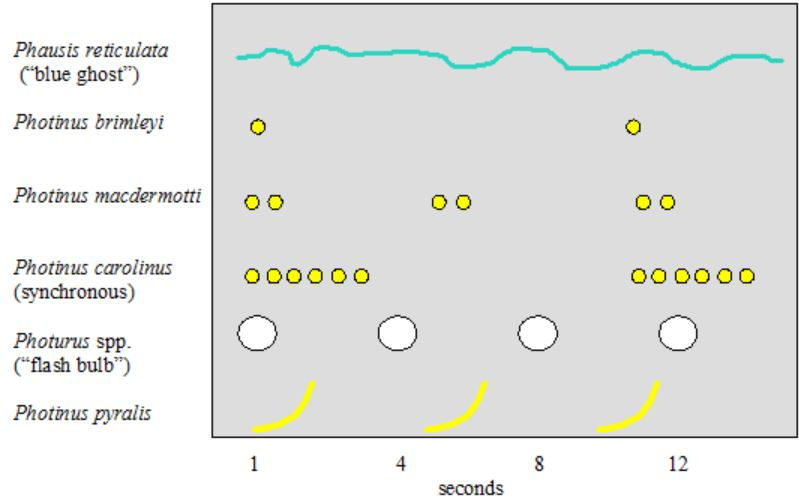
\includegraphics[width=\textwidth]{imgs/flash}
	\caption{Behaviour of fireflies flashing over the time. }
	\label{fig:intro_flash}
\end{figure}
 
The light patterns of fireflies are part of a mating display that the male fireflies use to attract the female ones. If successful, the female replies back with a characteristic flash of it own. Although this is synchronisation on its own, there are a few species of fireflies where more than 2 individuals can synchronize. These species are usually observed in large groups, all flashing together in unison.

As we can see in Figure~\ref{fig:intro_flash}, all of the species fire of one after another in a synchronized fashion except the blue one which seems to be random. 

\subsection{Goal}
Our goal for this study is to investigate Kuramoto oscilators with negative coupling co-efficients. We will define what exactly a coupling coefficient is and what negative coefficients mean in the next section, but one can intuitively think of it as a number measuring the strength of attraction between two oscilators. 
The reason we specifically want to use negative coupling coefficients is because, in contrast to positive coefficients, it is much easier to generate complex synchronisation patterns. We want to study and observe these patterns and investigate if we can construct systems that generate desired patterns. 

In Section~\ref{sec:kuramoto} we will introduce the Kuramoto oscillator, explain its equations, some required background knowledge as well as our implementation of it. In Section~\ref{sec:negative} we continue with describing the patterns we encountered when using negative coefficients. We then move on to describe a method which can be used to re-create arbitrary patterns in Section~\ref{sec:patterns} before concluding in Section~\ref{sec:conclusion}. 
	\newpage
	
	% Section 2
	\section{The Kuramoto oscilator}
	\label{sec:kuramoto}

The problem of having a naive viewpoint on the subject of synchronization is that one may believe that every different coupling situation would require its own treatment. This may stem from the fact that one may be focusing too much on the differences rather then the similarities which are found in all synchronous systems.  In this project we want to use the model of oscilators that was first introduced by Kuramoto in ~\cite{book:kura}. The most common form is given by the following system of ODEs:
\[
\dot{\theta_i} = \omega_i + \sum_{j = 0}^{N - 1}{A_{i, j}\sin({\theta_j - \theta_i}}) + b_i \sin(\Omega(t) - \theta_i)
\]
In this equation
\begin{itemize}
	\item $\theta_i$ is the phase of the $i\textsuperscript{th}$ oscillator, 
	\item $N$ the number of oscilators, 
	\item $\omega_i$ is the natural frequency of the $i\textsuperscript{th}$ oscillator, 
	\item $A$ is the matrix of coupling coefficients of the system, 
	\item $\Omega(t)$ is the phase of an external driver to the system and
	\item $b$ is the vector of coupling coefficients to the external driver
\end{itemize}

In the Kuramoto oscilator model the main object of study is the phase of $N$ different so-called Kuramoto oscilators, $\theta_0$ to $\theta_{N - 1}$. It should be noted that one usually looks at this modulo $2 \pi$. 

Each oscilator oscilates at its own natural frequency $\omega_i$. However they are also influenced by the different other oscilators as well as by an external driver to the system. The observation of the other oscilators is represented by the periodic $\sin$ function. How strong each oscilator is influenced by the others and the external drivers is measured by the so-called coupling coefficients $A_{i, j}$ and $b_i$ respectively. 

\subsection{The Coupling matrix and associated network topology}

We can easily see from the notation above that we can consider the coupling coeffients $A_{i, j}$ as a square matrix $A$ of size $N$. Similarly we can consider the coupling to the external driver as a vector $b$ of length $n$. 

It turns out that if we take a symmetric matrix $A$ the system exhibits very interesting behaviour that can be related to another interpretation of $A$. A symmetric matrix containing only zeros and ones can naturally be seen as the adjacency matrix of an undirected, finite graph. In an adjacency matrix the elements indicate whether pairs of vertices are connected via an edge or not, i.e. if the value is $1$ there is an edge, otherwise there is not. This information can then be used to reconstruct the graph from the matrix. 

When solving the system this natural interpretation of $A$ is very useful to understand the dynamics. A typical plot generated when simulating the system can be found in Figure~\ref{fig:adjacencymatrix}. On the top is the graph that is created from an adjacency matrix $A$. Each vertex of the system represents a single oscilator. On the bottom is a plot of the phases of the oscilators of the system over time. 

\begin{figure}[h]
\centering
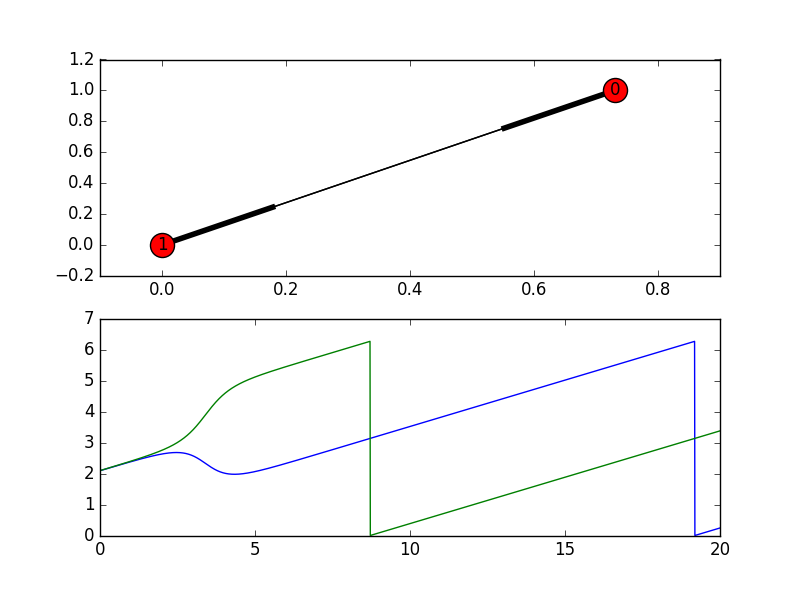
\includegraphics[width=\textwidth]{imgs/examplefigure}
\caption{A typical plot of a topology and output of the system}
\label{fig:adjacencymatrix}
\end{figure}

\subsection{Implementation of the system}
We have implemented a simulation of this system using Python3. Our implementation uses the python packages Numpy, Scipy and Networkx. In particular it leverages the standard ODE solver functionality provided by \lstinline{scipy.integrate.odeint}. Our code is very modular and consists of four distinct modules: 

\begin{enumerate}
	\item A simulator of the system, found in \lstinline{oscilator.py}. This takes the parameters for the ODE and runs a simulation of the system given some initial values. 
	\item Some plotting code, found in \lstinline{plotter.py}, which takes the output of the system and makes plots like the ones that can be found in the various Figures in this report. 
	\item Some code that generates adjacency matrices for specific graphs, found in \lstinline{graph_generators.py}. 
	\item the main code of the system, found in \lstinline{code.py}, which utilises the components above and runs the entire simulation. 
\end{enumerate}

The gist of our simulation code happens in the line below. Here \lstinline{self.to_equation()} reads the current parameters and generates a function that directly represents the ODE we want to solve. To improve performance, this compiles a string of python code at runtime to a function. This is then used together with initial values \lstinline{y0} and times \lstinline{t} to simulate the ODE for and passed to the \lstinline{odeint} function. 

\begin{lstlisting}
sol = odeint(self.to_equation(), y0, t, *args, **kwargs)
\end{lstlisting} 

In order to interpret the matrix $A$ as a graph, we use the networkx library and a slightly adapted version of the code below. 

\begin{lstlisting}
# create a new graph
G = nx.DiGraph()

# read current parameters
A = self.A
N = self.N

# add all the edges
for i in range(N):
		for j in range(N):
				if A[i, j] != 0:
						G.add_edge(i, j, weight=A[i,j])

# and return the graph
return G
\end{lstlisting}

Finally to generate Figures such as Figure~\ref{fig:adjacencymatrix}, we then plot this graph together with the solution provided by odeint.  
	\newpage
	
	% Section 3
	\section{Patterns in negative coefficient systems}
	\label{sec:negative}
For our investigation of the negative coefficient situation we consider a simplified version of the Kuramoto oscilator. Specifically we assume that all oscilators have the same basic frequency $\omega_i$, which we just call $\omega$. We also assume that there is no external driver to the system, i.e. $b_i = 0$. This simplifies the system of ODEs to: 

\[
\dot{\theta_i} = \omega + \sum_{j = 0}^{N - 1}{A_{i, j}\sin({\theta_j - \theta_i})}
)\]

Furthermore we assume that all coefficients in the matrix $A$ are either $-1$ or $0$. We can thus see $A$ as the negative of an adjacency matrix of a graph. Here each oscilator is considered as a node of a graph and an edge can be interpreted as $A$ having a $-1$ in the appropriate place. 

\subsection{The 2-oscilator system}

The first situation we consider is the case of only $2$ oscilators. It is obvious that if the oscilators are not connected through an edge, no synchronization occurs. Thus the only situation of interest is the case where they are connected through an edge, i.e. 
\[
  A = \left( \begin{array}{cc} 0 & -1\\ -1 & 0 \end{array} \right)
\]
We have simulated this situation with random initial values for the oscilators. As can be seen from the typical result in Figure~\ref{fig:negative_2_osc} the two oscilators lock to the same frequency but have a phase shift of $\pi$, i.e. they are in anti-phase. We observed that this behaviour occurs independent of the initial values. This behaviour stems from the fact that the two oscilators are influencing each other with equal negative coefficients and thus want to oscilate as far away from each other as possible. 

\begin{figure}[h]
  \centering
  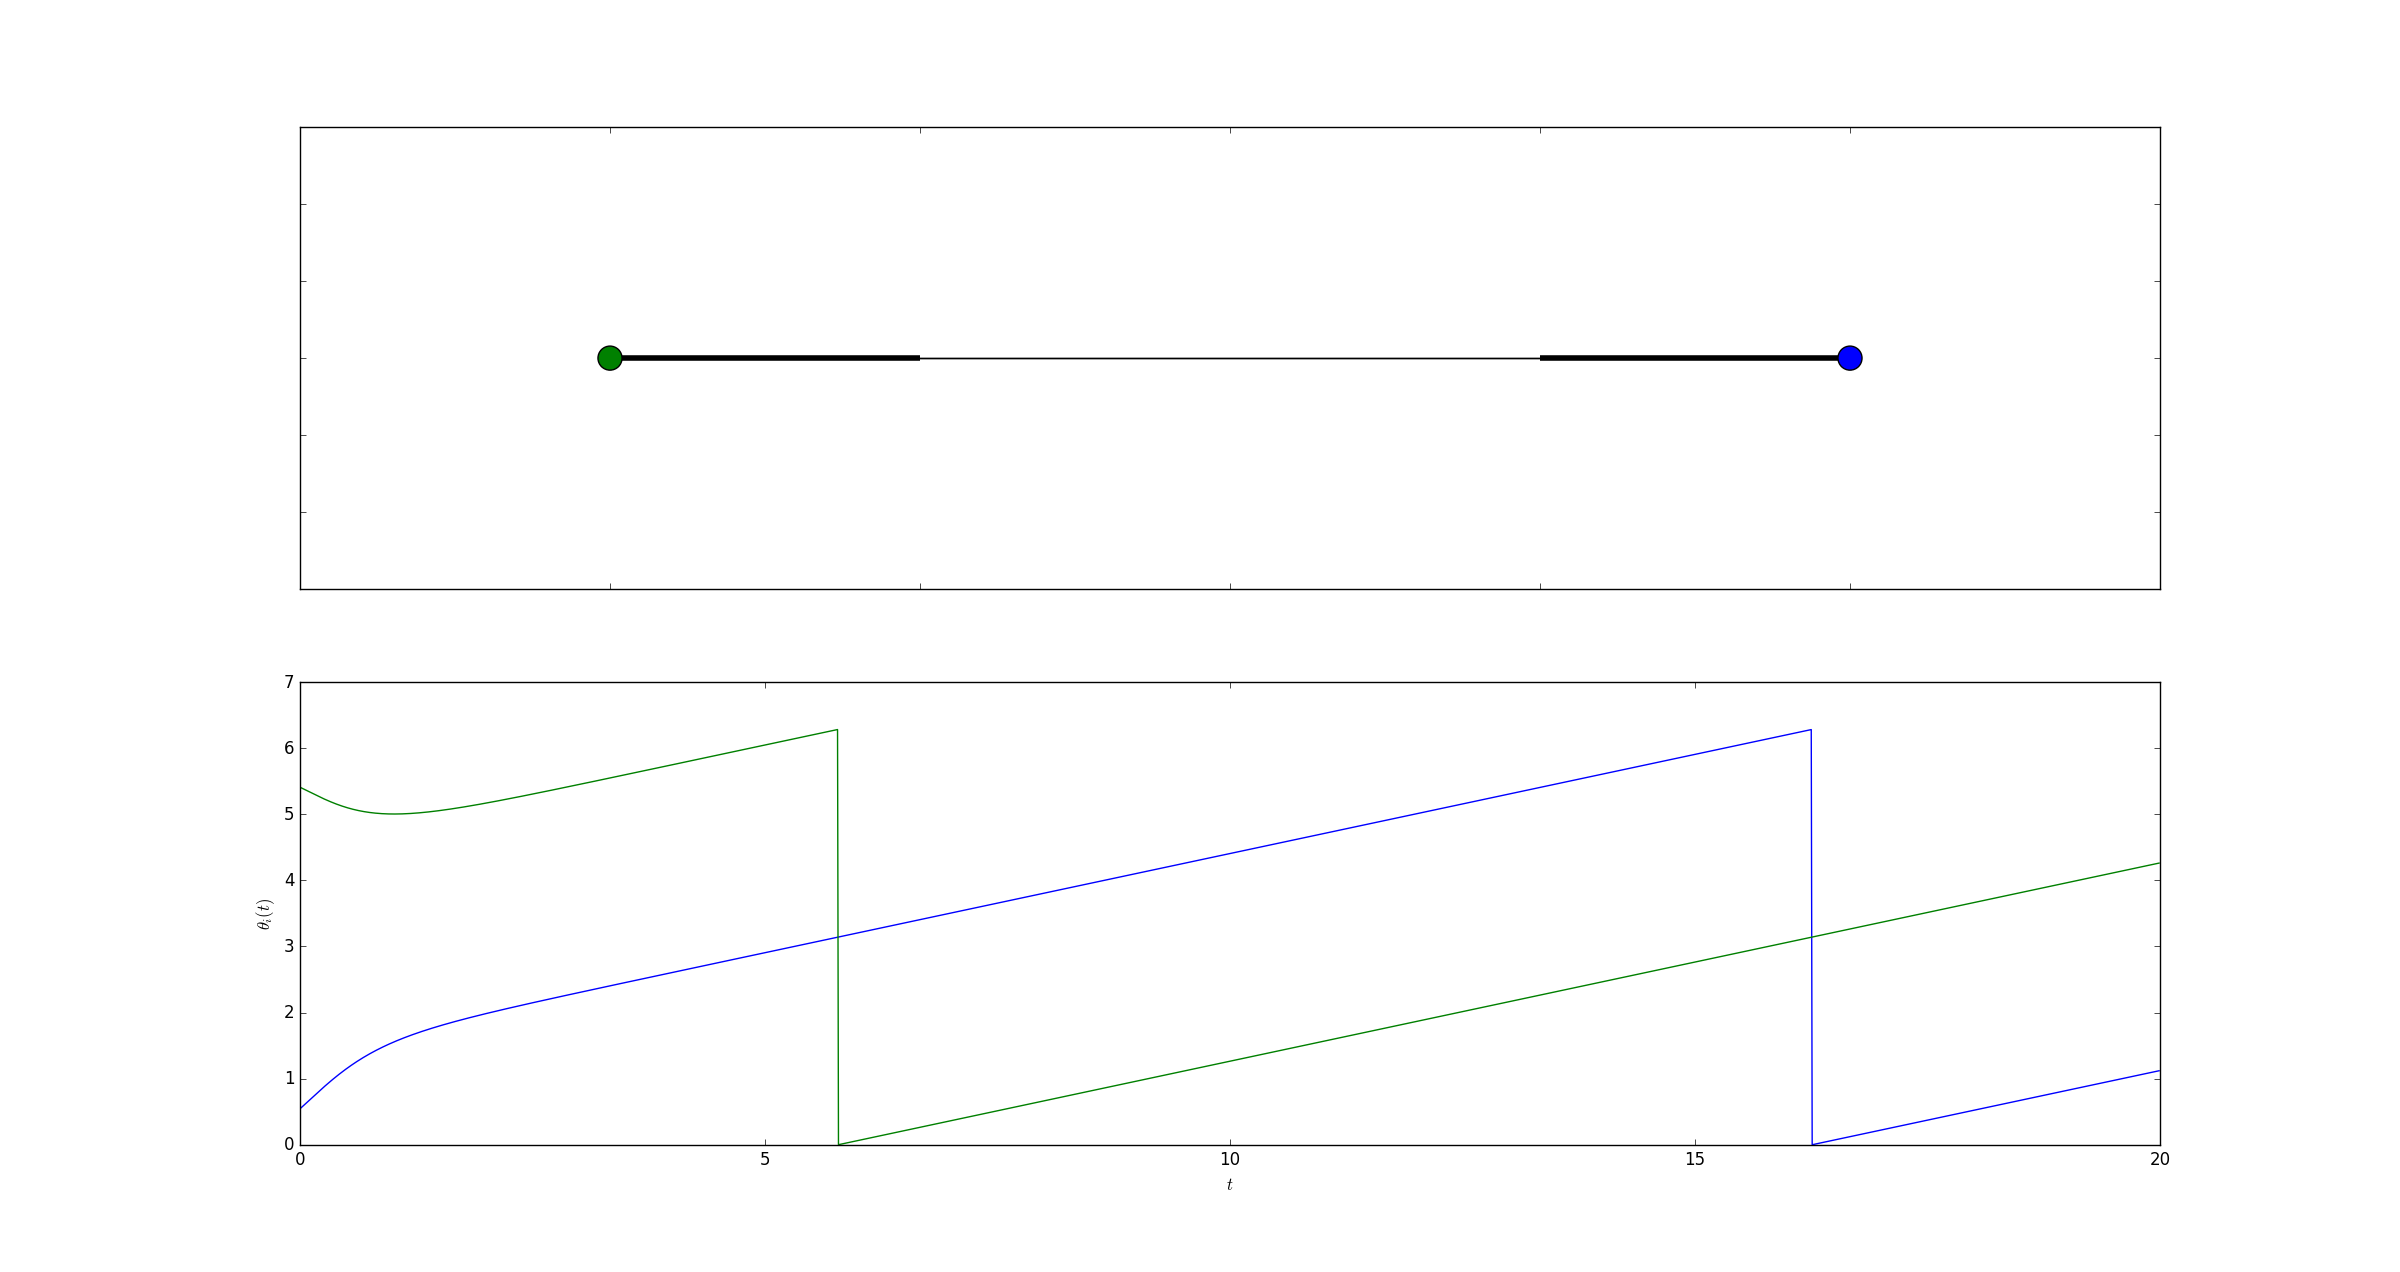
\includegraphics[width=\textwidth]{imgs/simple_2_osc}
  \caption{Simulation of a simplified 2 oscilator Kuramoto system with $\omega = 0.3$ and random initial values. $A$ is given by the negative of the adjacency matrix of the associated graph topology which can be seen in the upper part of the figure. The behaviour of the oscilators over time can be seen in the lower part. }
  \label{fig:negative_2_osc}
\end{figure}

\subsection{Oscilators on a line}

Next we want to expand this behaviour to the situation of several oscilators on a line. In this sense, that refers to the situation where $N$ oscilators are ordered linearly and each oscilator is only connected to the next and previous in the line with the exception of the ones at either end of the line. The associated matrices $A$ to these situations are $0$ except as two bands above and below the diagonal.  

In the case of three oscilators the adjacency matrix is given by
\[
  A_3 = \left( \begin{array}{ccc}
  0  & -1 &  0\\ 
  -1 &  0 & -1
  \end{array} \right)
\] 
and in the case of 10 oscilators it is given by
\[
  A_{10} = \left( \begin{array}{cccccccccc}
  0 & -1 & 0 & 0 & 0 & 0 & 0 & 0 & 0 & 0 \\
  -1 & 0 & -1 & 0 & 0 & 0 & 0 & 0 & 0 & 0 \\
  0 & -1 & 0 & -1 & 0 & 0 & 0 & 0 & 0 & 0 \\
  0 & 0 & -1 & 0 & -1 & 0 & 0 & 0 & 0 & 0 \\
  0 & 0 & 0 & -1 & 0 & -1 & 0 & 0 & 0 & 0 \\
  0 & 0 & 0 & 0 & -1 & 0 & -1 & 0 & 0 & 0 \\
  0 & 0 & 0 & 0 & 0 & -1 & 0 & -1 & 0 & 0 \\
  0 & 0 & 0 & 0 & 0 & 0 & -1 & 0 & -1 & 0 \\
  0 & 0 & 0 & 0 & 0 & 0 & 0 & -1 & 0 & -1 \\
  0 & 0 & 0 & 0 & 0 & 0 & 0 & 0 & -1 & 0
  \end{array} \right)
\]
The typical behaviour of such systems can be seen in Figures~\ref{fig:line_3} and \ref{fig:line_10} respectively. The behaviour naturally extends the behaviour of the 2 oscilator systems above: Neighbouring oscilators are in exact anti-phases. Experiments showed this behaviour to be independent of initial values and the number of oscilators, although the higher the number of oscilators, the longer the system needs to reach this state. 

\begin{figure}[h]
  \centering
  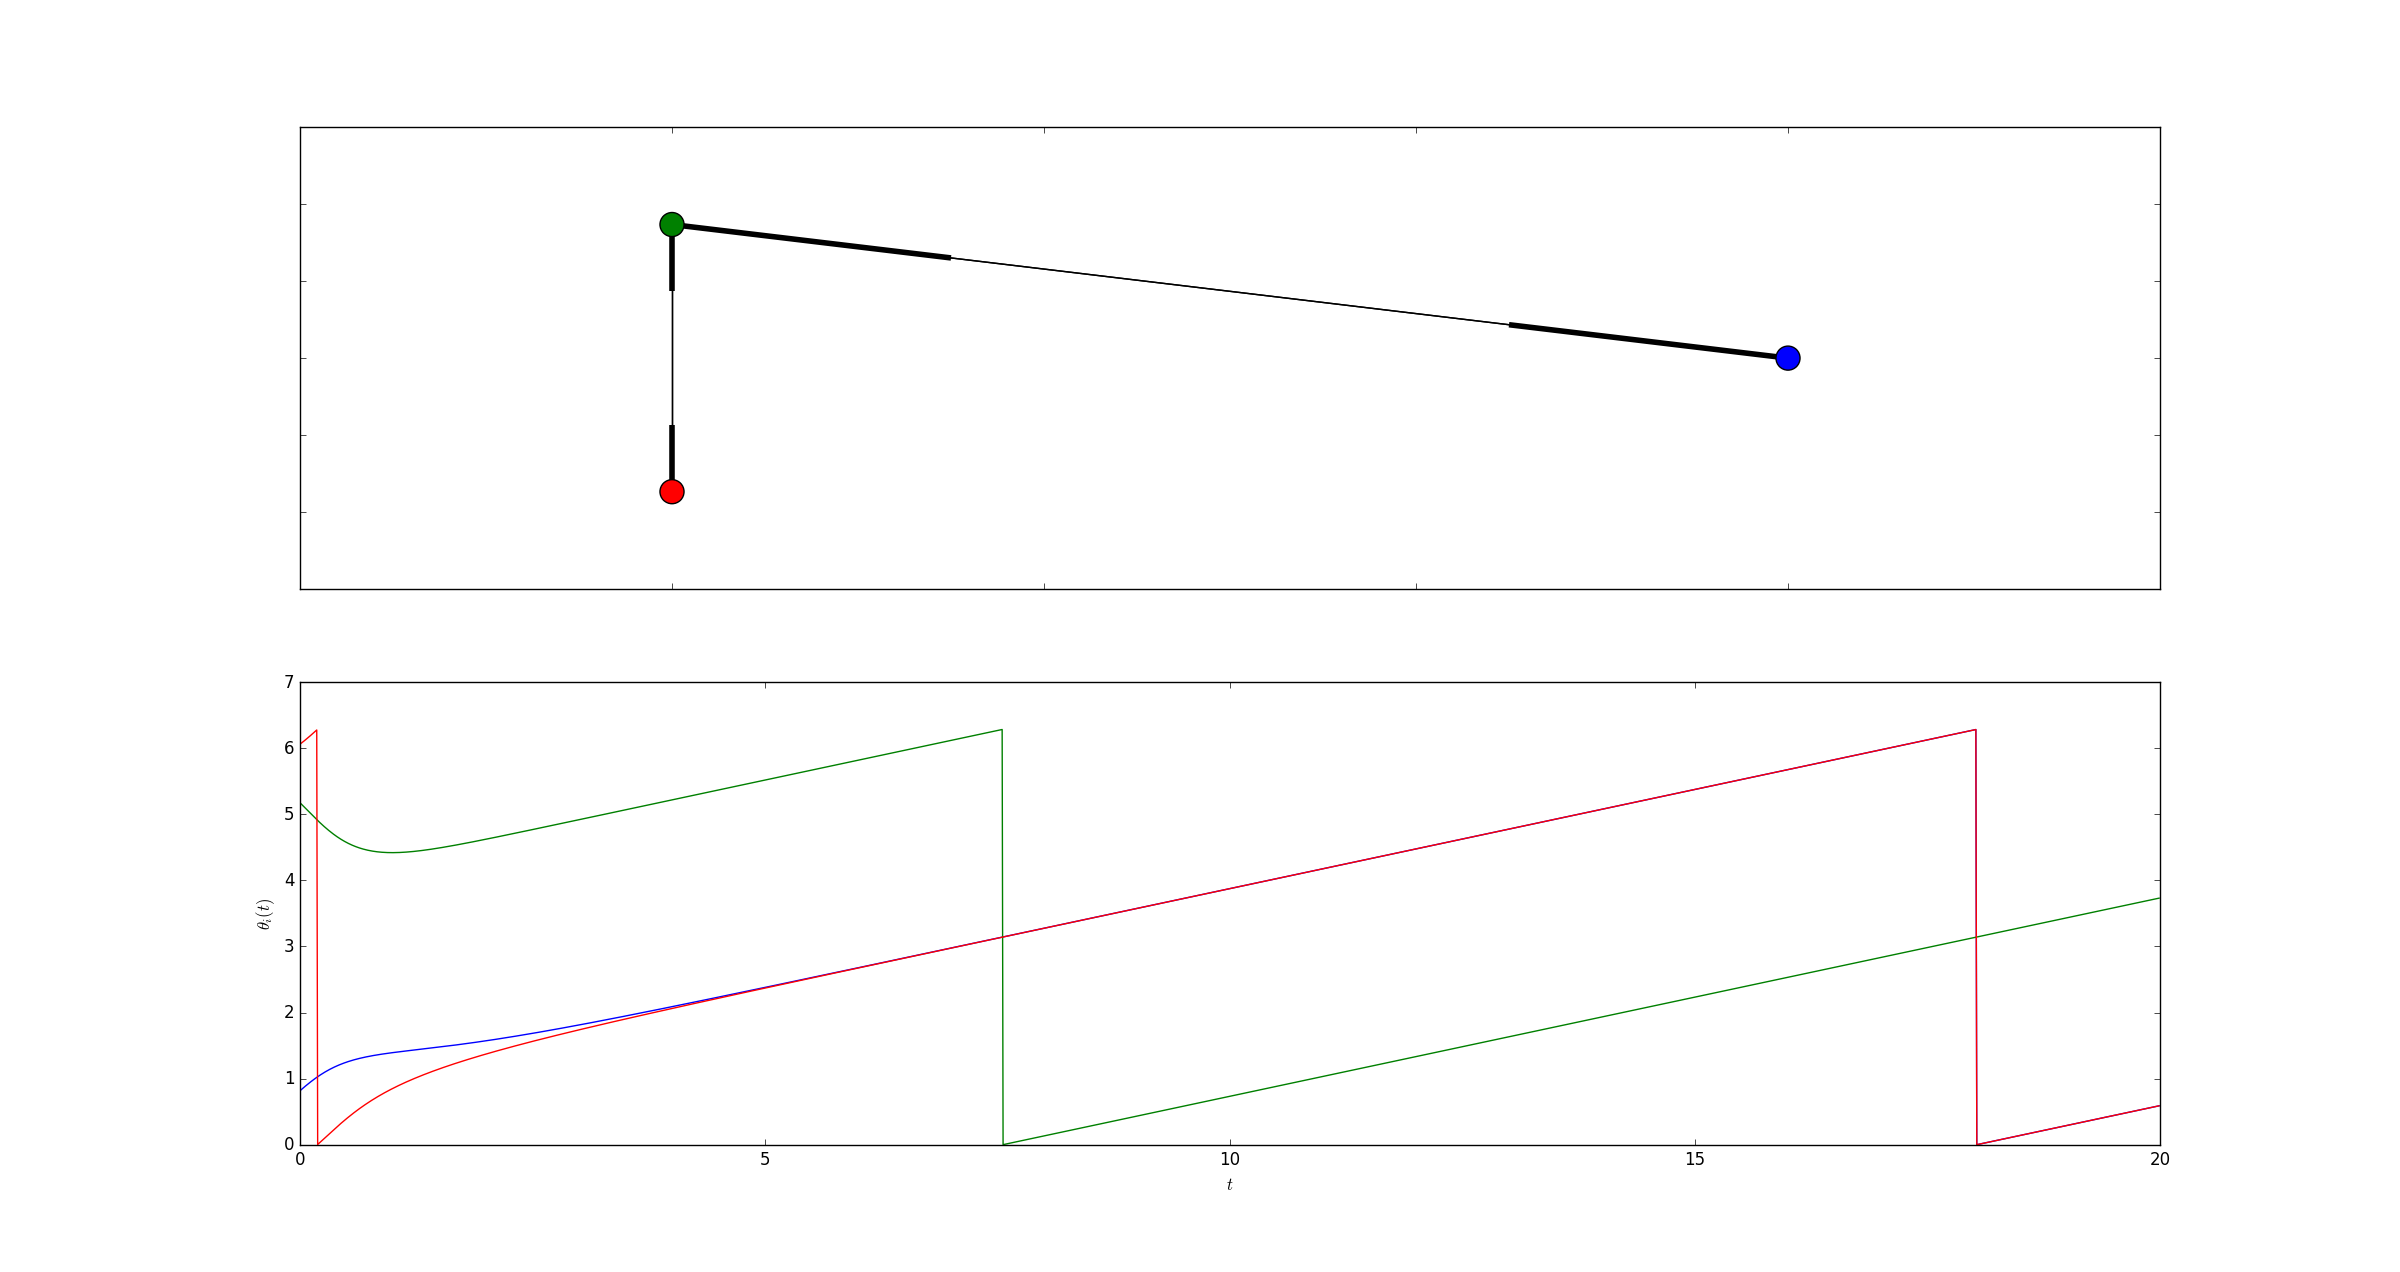
\includegraphics[width=\textwidth]{imgs/line_3}
  \caption{Simulation of a 3 oscilators-on-a-line Kuramoto oscilator system with $\omega = 0.3$ and random initial values. Again $A$ is given by the negative of the adjacency matrix of the associated graph topology. }
  \label{fig:line_3}
\end{figure}

\begin{figure}[h]
  \centering
  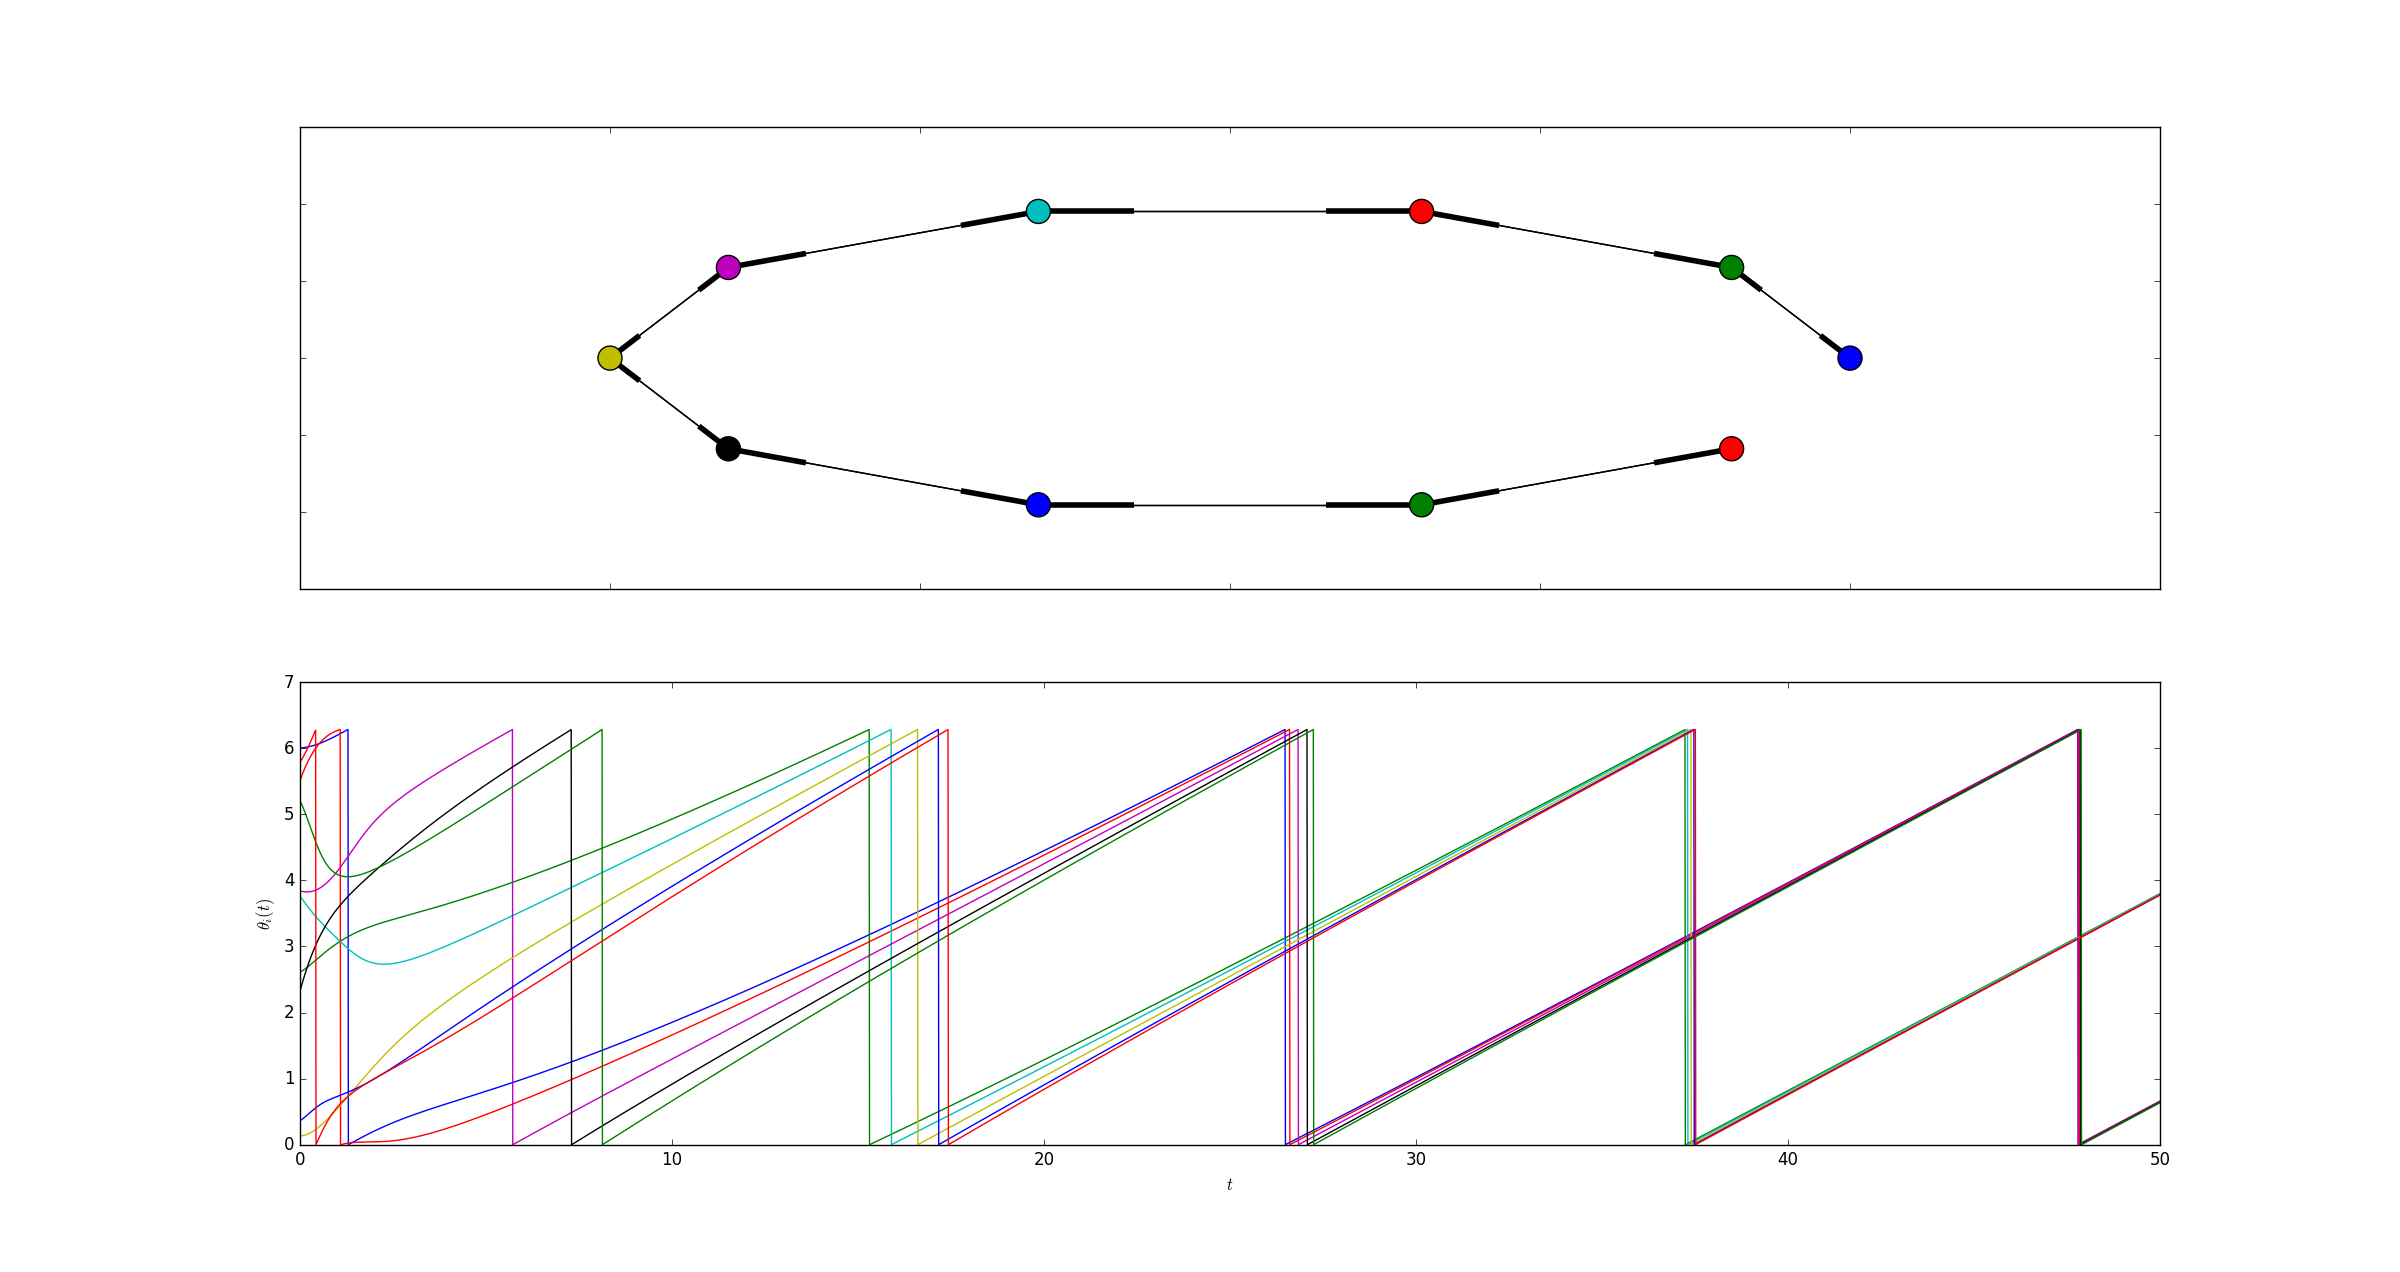
\includegraphics[width=\textwidth]{imgs/line_10}
  \caption{Simulation of a 10 oscilators-on-a-line Kuramoto oscilator system with $\omega = 0.3$ and random initial values. Again $A$ is given by the negative of the adjacency matrix of the associated graph topology. }
  \label{fig:line_10}
\end{figure}

\subsection{Oscilators on a Circle System}

The final patterns we observed were patterns in the case of $N$ oscilators on a cycle. This graph looks very similar to the oscilators-on-a-line situation except that the first and last nodes are connected via an edge as well. We have again simulated the system and in this situation we came to interesting results. In the case of $3$ oscilators on a cycle (which can be seen in Figure~\ref{fig:circle_3}) the behaviour is obvious: The oscilators synchronize with phase-shits of exactly $\frac{2 \pi}{3}$. 

\begin{figure}[h]
  \centering
  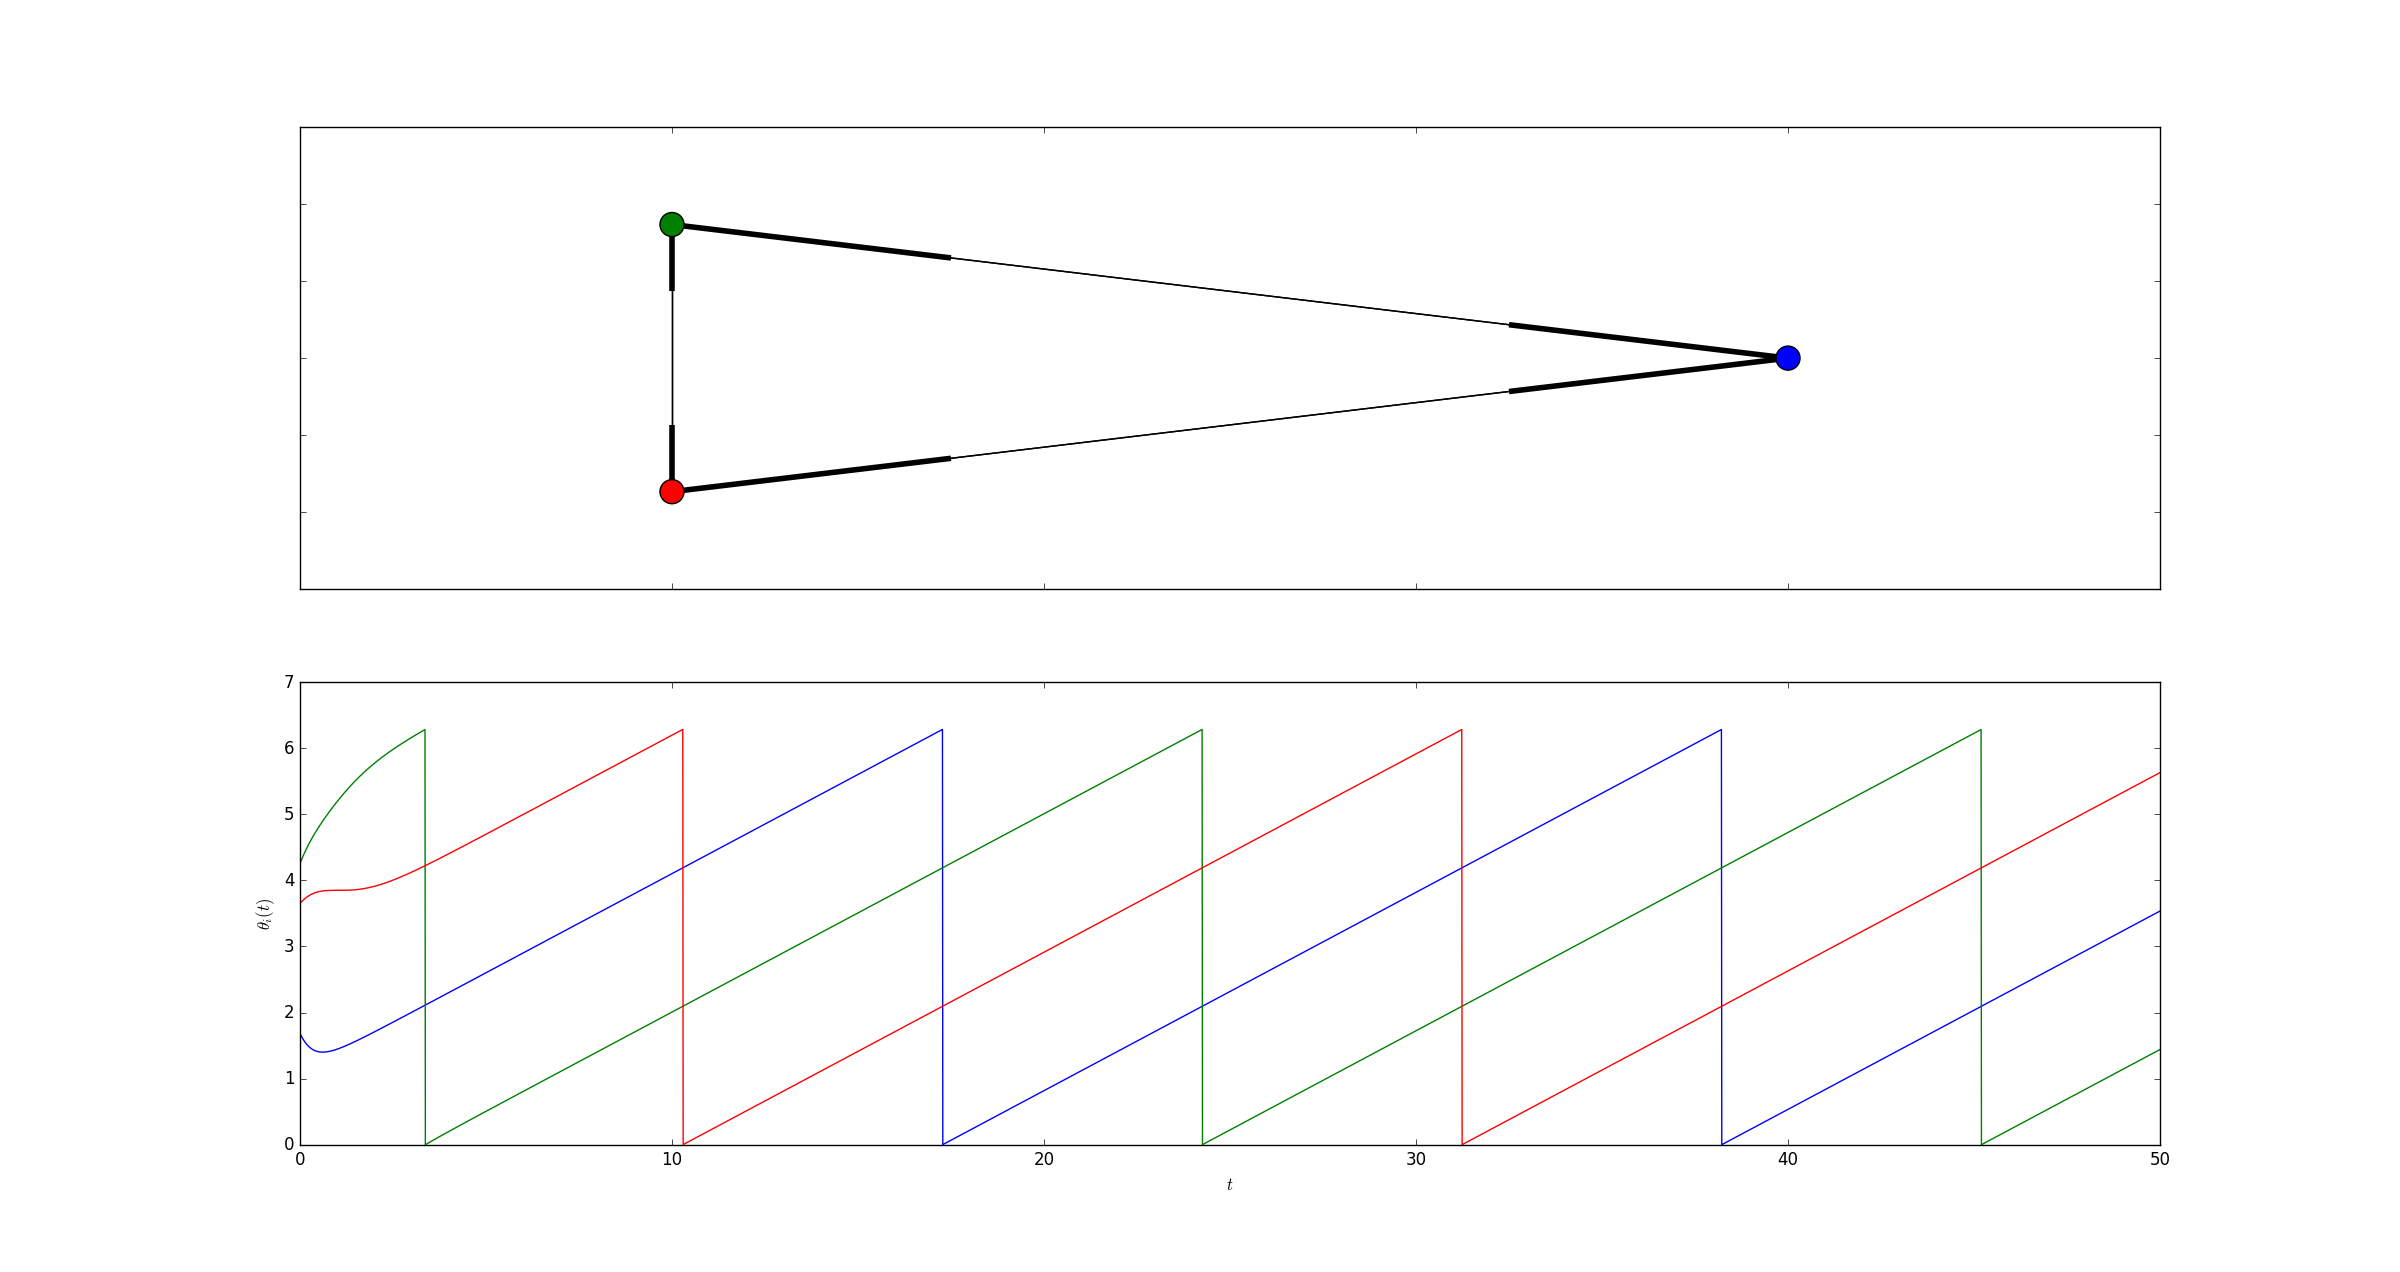
\includegraphics[width=\textwidth]{imgs/circle_3}
  \caption{Simulation of a 3 oscilators-on-a-circle Kuramoto oscilator system with $\omega = 0.3$ and random initial values. Again $A$ is given by the negative of the adjacency matrix of the associated graph topology. }
  \label{fig:circle_3}
\end{figure}

The behaviour becomes more interesting however if we choose a different number of oscilators, for example $6$. In this case we observed three different situations with three different kinds of phase shifts: Either phase shifts of $\pi$ (nodes with distance 2 were exactly in phase, see Figure~\ref{fig:circle_6a}), phase shifts of $\frac{2 \pi}{3}$ (nodes with distance 3 were exactly in phase, see Figure~\ref{fig:circle_6b}) or phase shifts of $\frac{2 \pi}{6}$ (see Figure~\ref{fig:circle_6c}). The last of these patterns could only be produced artificially by choosing the desired situation as initial values and proved to be very unstable. 

\begin{figure}[h]
  \centering
  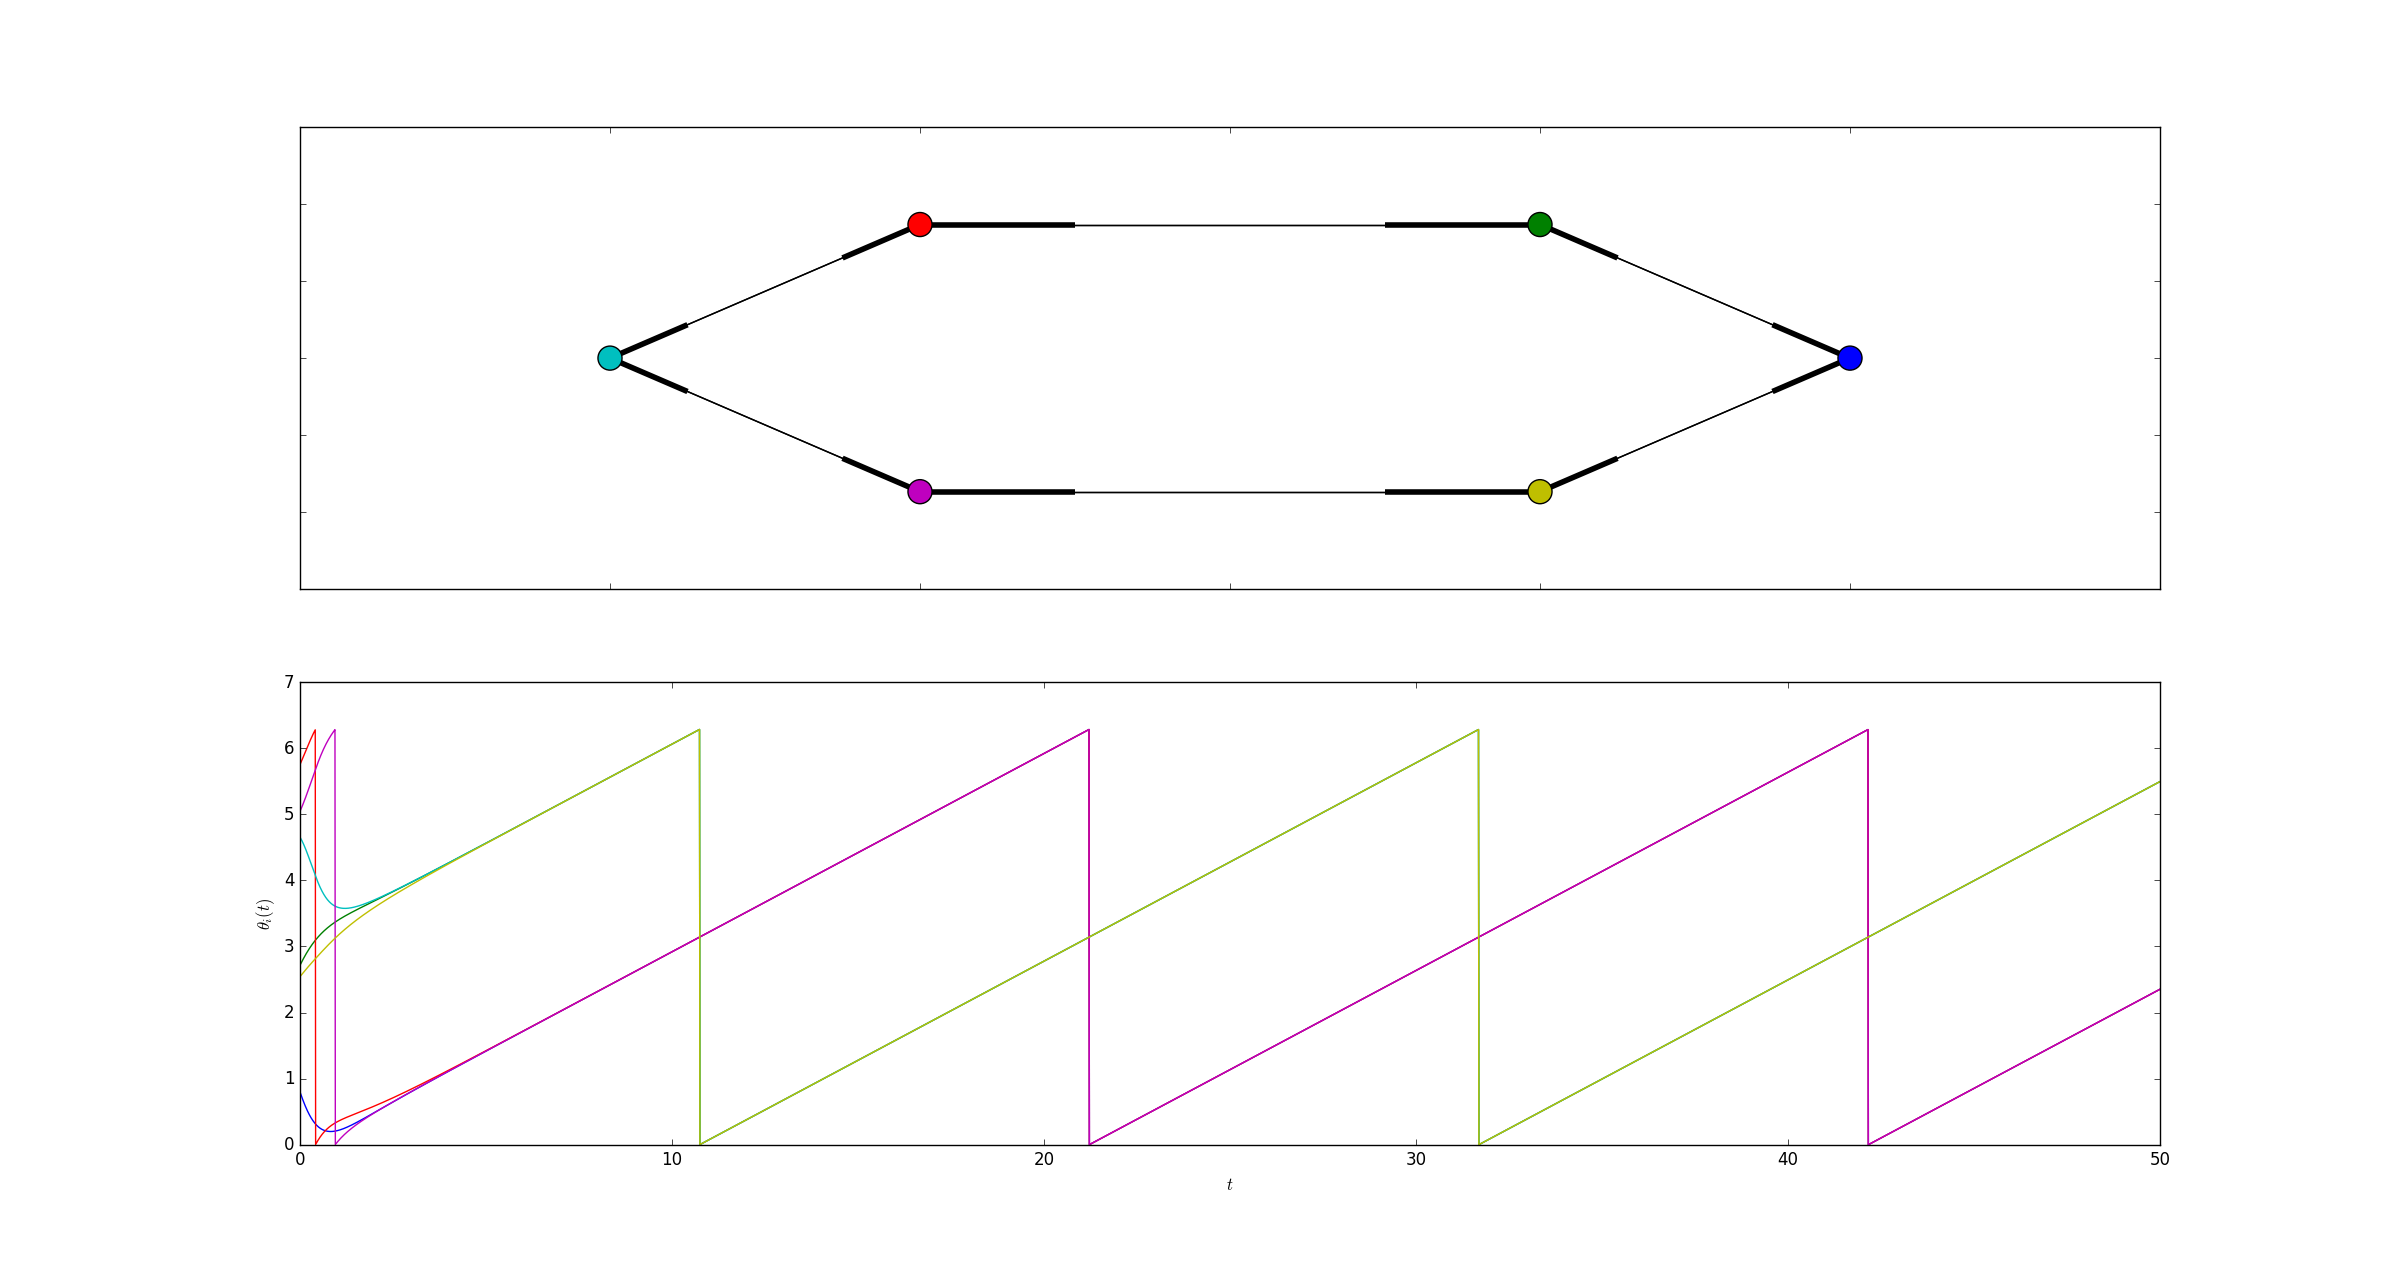
\includegraphics[width=\textwidth]{imgs/circle_6a}
  \caption{Simulation of a 6 oscilators-on-a-circle Kuramoto oscilator system with $\omega = 0.3$ and random initial values producing a pattern of neighbouring oscilators being exactly anti-phase}
  \label{fig:circle_6a}
\end{figure}

\begin{figure}[h]
  \centering
  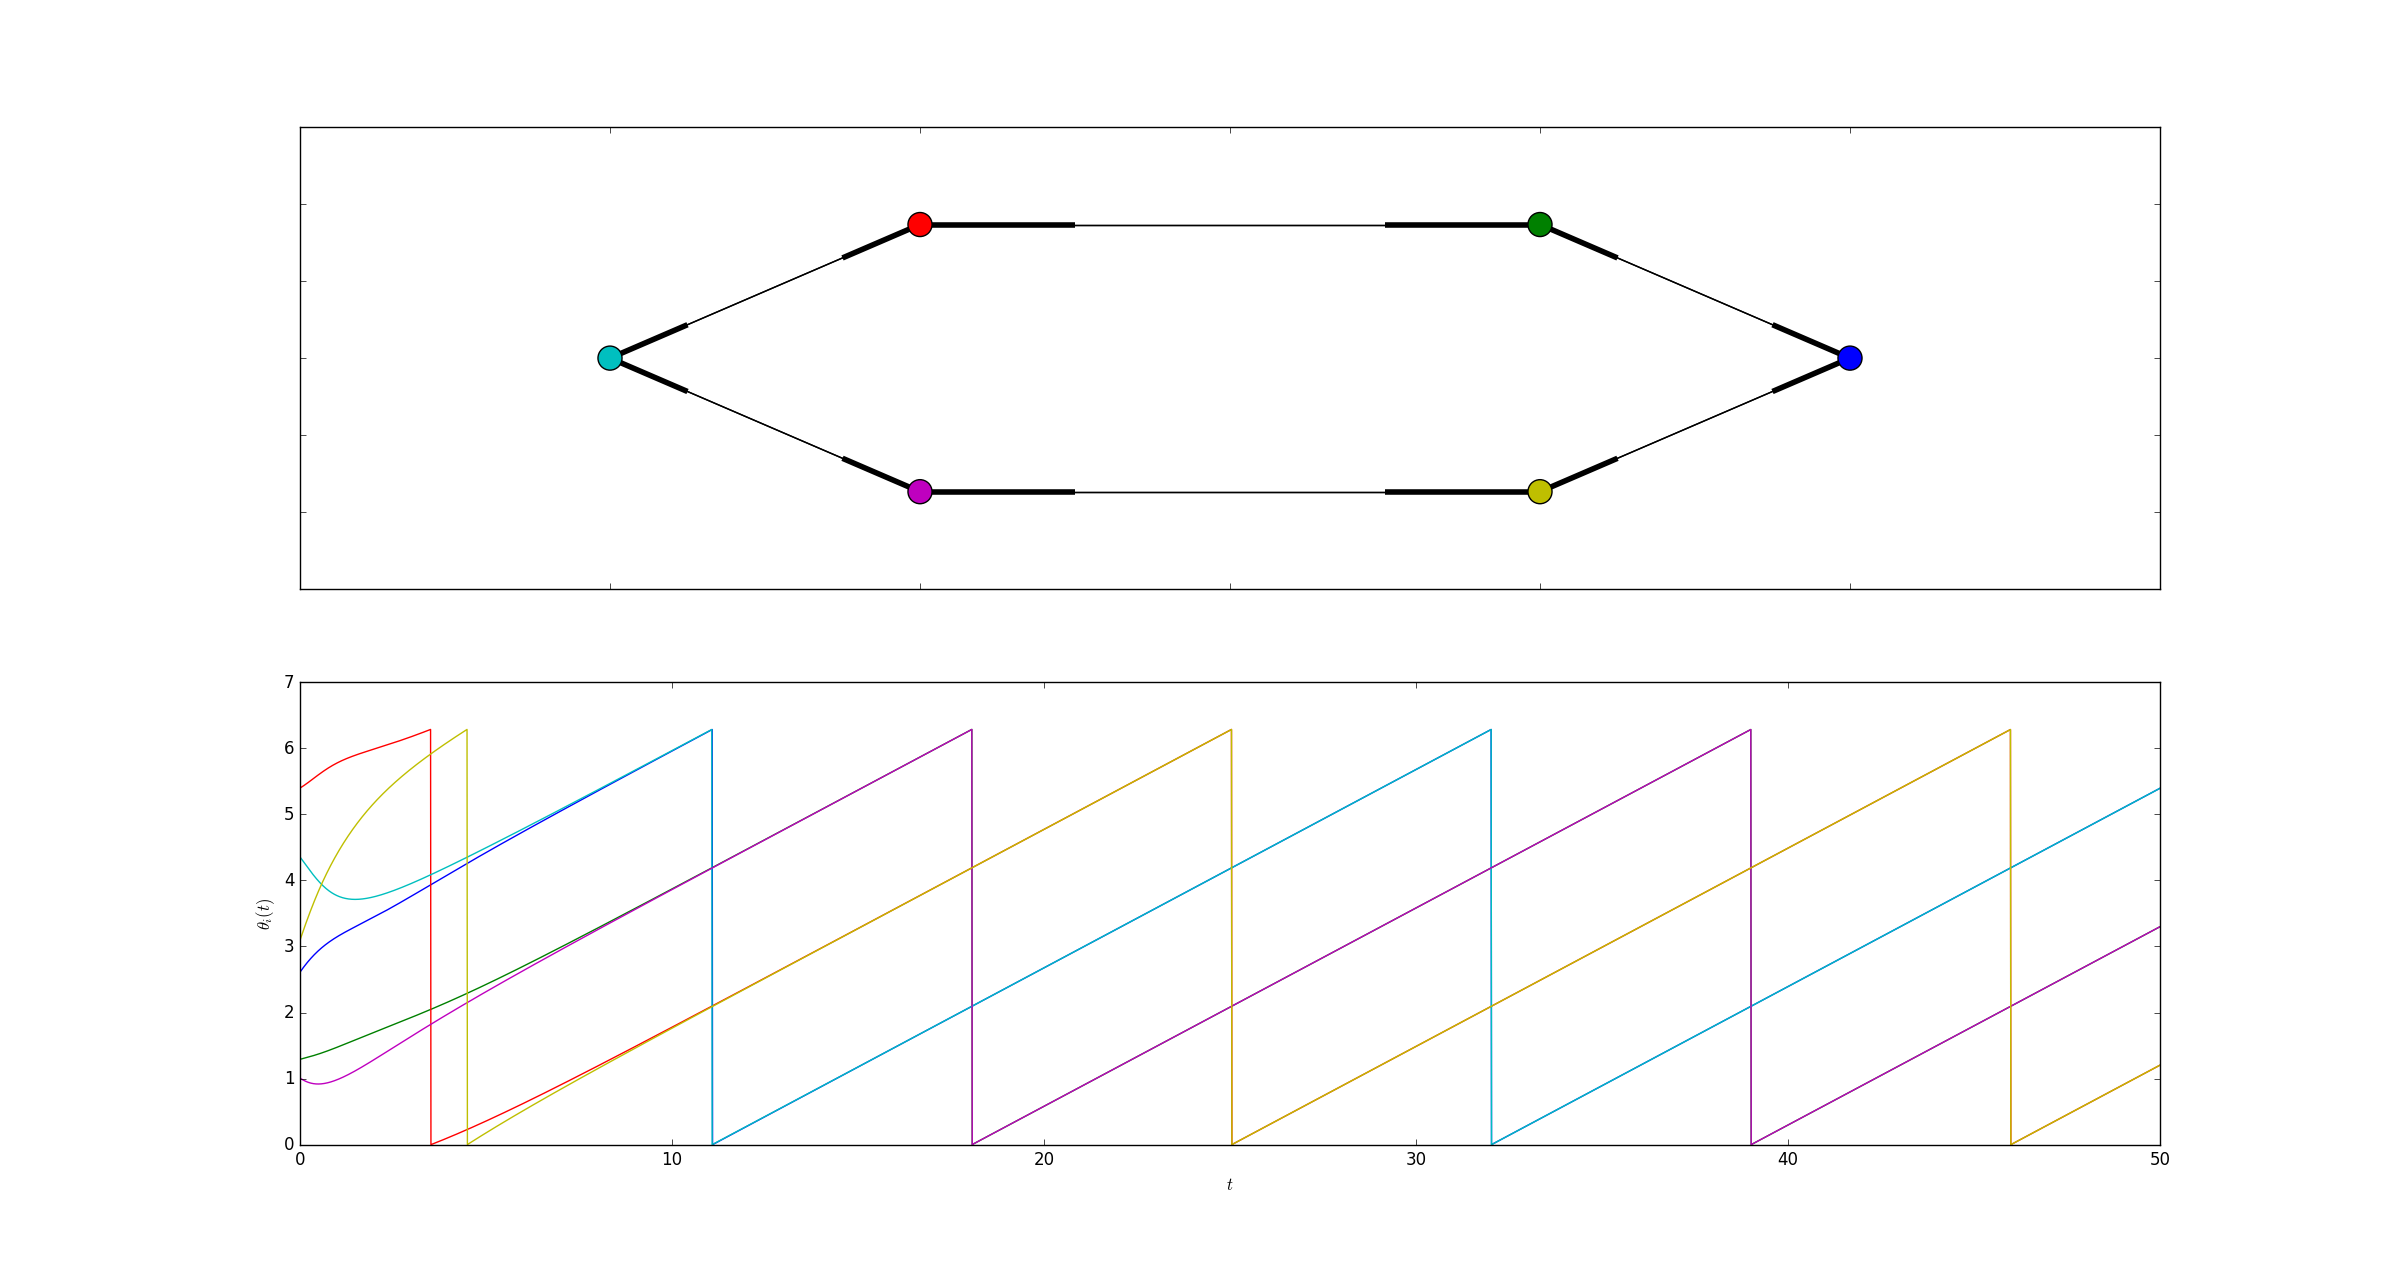
\includegraphics[width=\textwidth]{imgs/circle_6b}
  \caption{Simulation of a 6 oscilators-on-a-circle Kuramoto oscilator system with $\omega = 0.3$ and random initial values priducing a pattern of every 3 oscilators being in sync. }
  \label{fig:circle_6b}
\end{figure}

\begin{figure}[h]
  \centering
  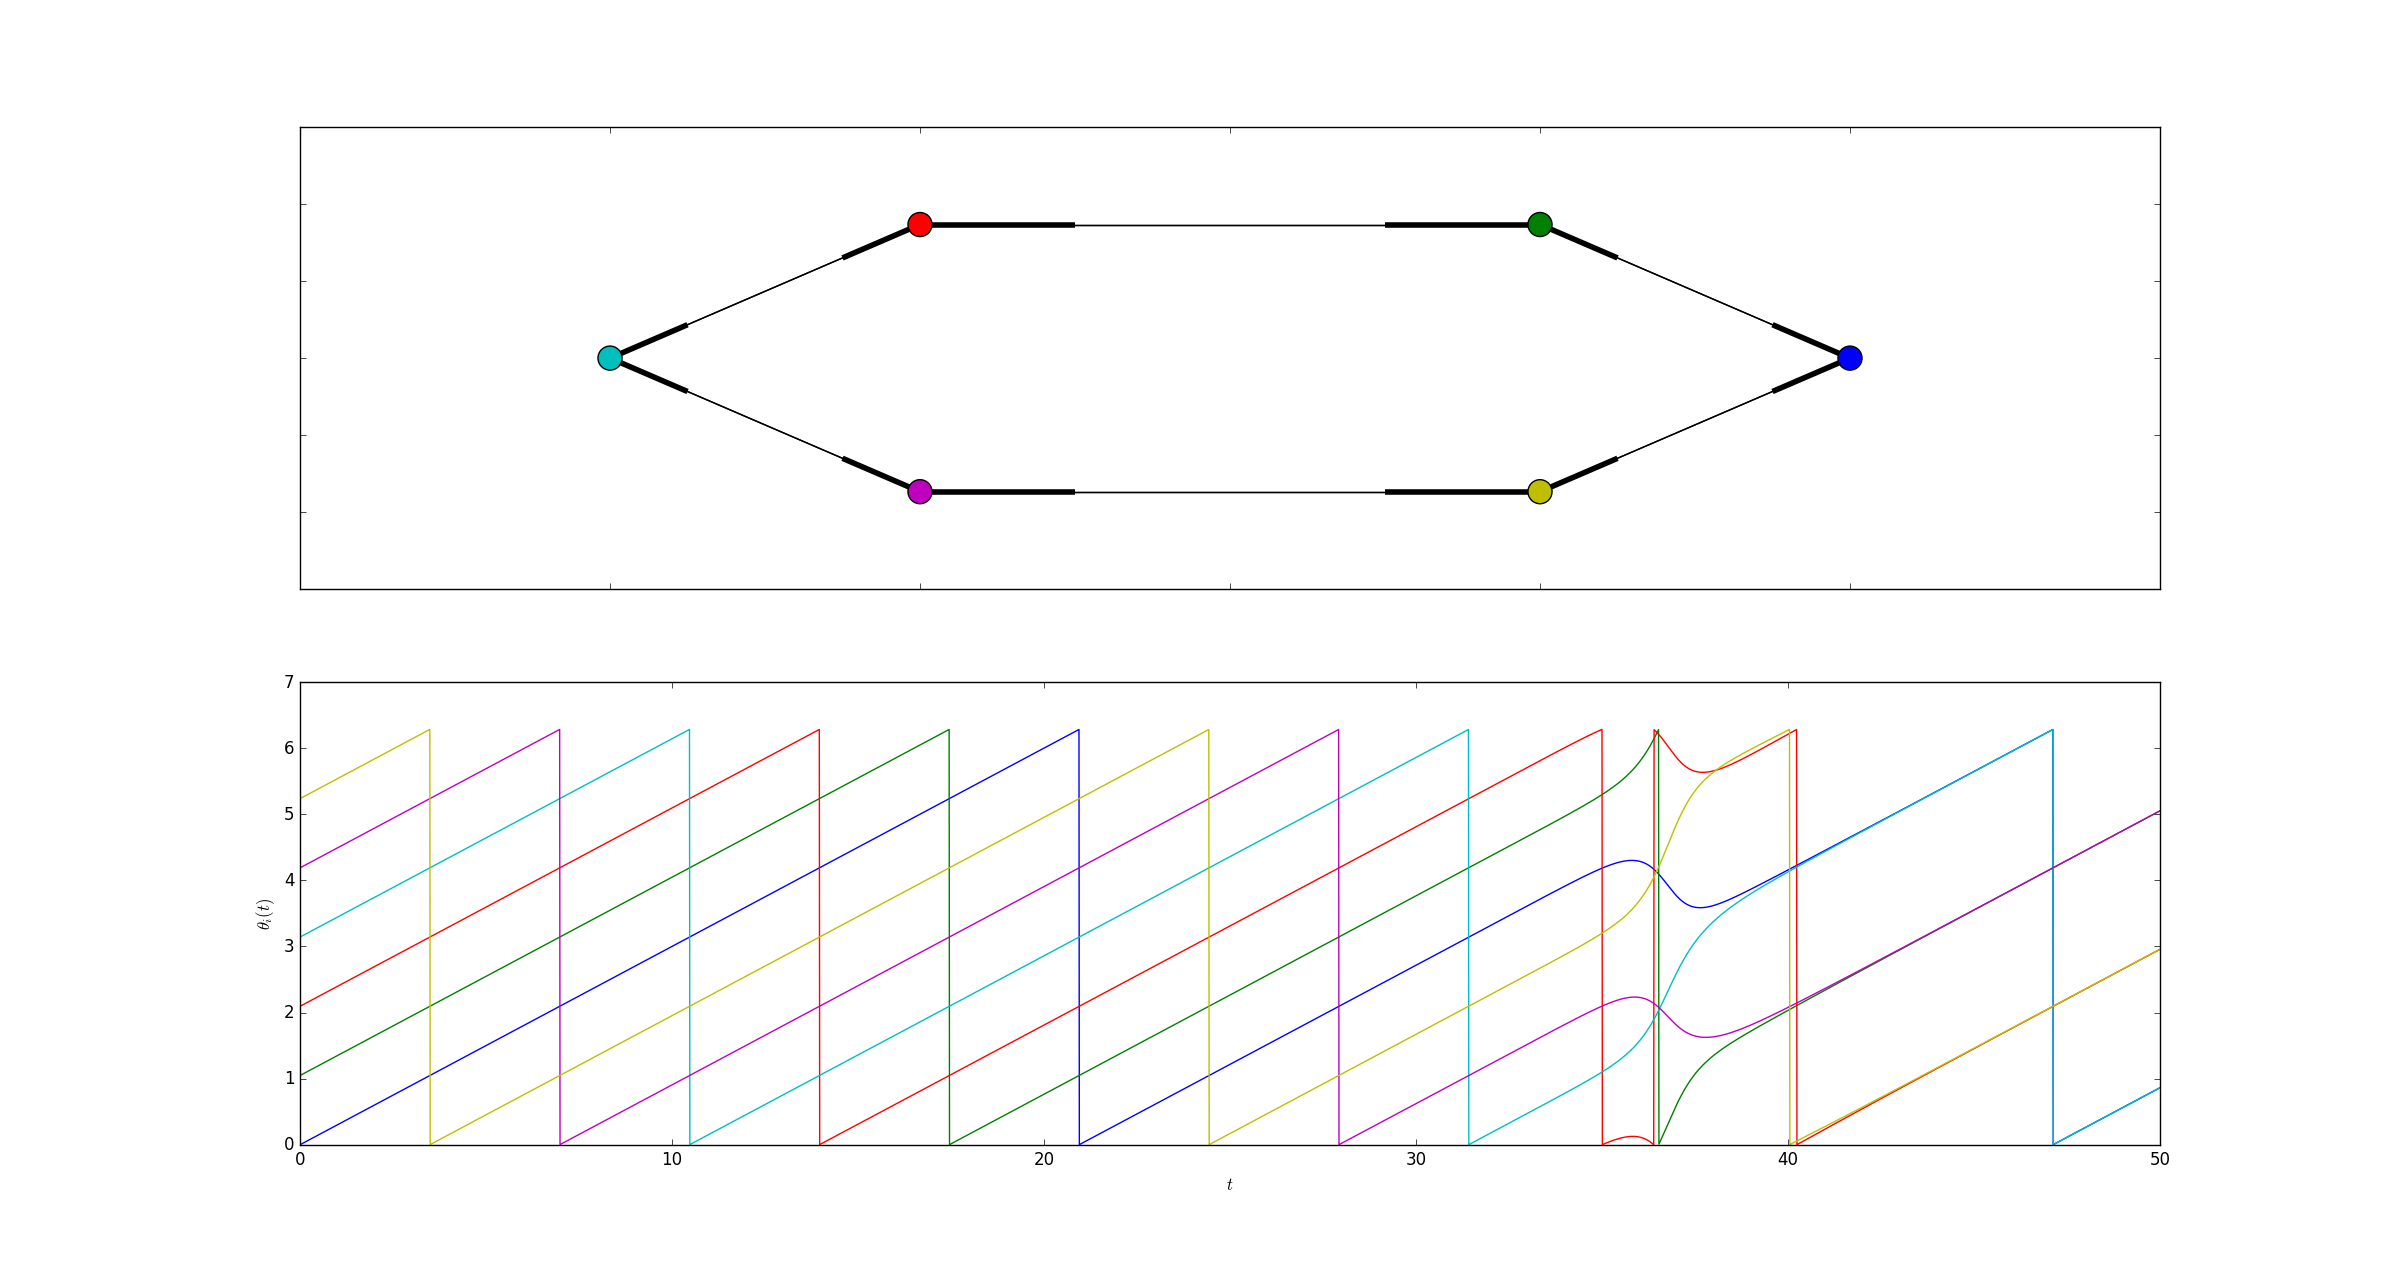
\includegraphics[width=\textwidth]{imgs/circle_6c}
  \caption{Simulation of a 6 oscilators-on-a-circle Kuramoto oscilator system with $\omega = 0.3$ and specific initial values producing an unstable pattern of oscilators being evenly spaced out in phase shifts. }
  \label{fig:circle_6c}
\end{figure}

From these patterns we can deduce that the possible patterns in the general case of $N$ oscilators-on-a-circle depends on the divisors of $N$. Since each oscilator wants to be as far away from its neighbours as possible, they space out equally with respect to their phase shifts. However since each oscilator has to be in phase with itself, the sum of all phase shifts around the cycle must be a multiple of $2\Pi$. Thus for each divisor of $N$ we get a different pattern, which is exactly what we observed. 
	\newpage
	
	% Section 4
	\section{Reproducing desired patterns}
	\label{sec:patterns}

\subsection{Defining pattern reproduction}

After making the observations in the previous section the next question that naturally occurs is if given a certain pattern, is there an associated graph topology (or associated matrix $A$) that is capable of reproducing it? In other words given a pattern, can we ``train'' a topology to create it?

In order to answer this question we first need to define ``pattern'' properly. We consider a pattern as the set of phase shifts between the different Kuramoto oscilators. In order to be able to observe a pattern it is neccessary for the oscilators to either have the same intrinsic frequencies $\omega_i$ or lock into the same frequency. In our case we just consider the first case. 

The reader should furthermore note that since we only consider phase shifts, the order of oscilators themselves is not relevant and all observation should be invariantmodulo $2\pi$. 

\subsection{Simple patterns}

We shall first consider the simple case of reproducing a simple pattern between 2 oscilators. If we take into account what we learned in the previous section, it is easily possible to re-create phase-shifts of $\frac{2\pi}{p}$ when $p$ is prime. 

If we set up $p$ oscilators on a cylic graph, we can get different phase shifts between neighbouring oscilators. For each divisor $d \neq 1$ of $p$ we can achieve phase shifts of $\frac{2\pi}{d}$ between neighbouring nodes. However since $p$ is prime, there is only a single such divisor, namely $p$ itself, and we will always achieve a phase shifts of $\frac{2\pi}{p}$. 

There is a caveat to this situation: We now have $p$ different oscilators in our topology instead of just two. This is not a big problem however, we can just pick two oscilators at random and ignore the others. 

\subsection{Creating More Complex Patterns}

We now have the ability to create simple patterns by setting up oscilators in a cirle topology. Using the same topology we can also create offsets of the shape $\frac{a {\cdot} 2 \pi}{p}$ where $p$ prime and $a \in \mathbb{N}$. Instead of taking two neighbouring nodes, we can just take two nodes of distance $A$ on the same topology. 

This introduces yet another caveat to the situation: We know the phase shift difference between two values but we can not predict which one is of higher value and which one is of lower value. Since we are working modulo $2 \pi$ this is not even well defined. 

But how can we expand this behaviour to reproduce any phase shifts $\frac{p {\cdot} 2 \pi}{q}$ with $p, q \in \mathbb{N}, q \neq 0$? Turns out it is possible to ``add'' phase shifts by joining two cicular toplogies. Both circles will behave as they would individually and additionally the node at which they are joined will always have the same value. 

If we wanted to for example reproduce the phase $\frac{8 {\cdot} 2 \pi}{15}$ we can use one circle of size $3$ and one circle of size $5$. Their phase shifts of $\frac{2\pi}{5}$ and $\frac{2\pi}{5}$ add up to $\frac{8 {\cdot} 2 \pi}{15}$, exactly what we want. The topology can bee seen in Figure~\ref{fig:pattern_joined}. 

\begin{figure}[h]
  \centering
  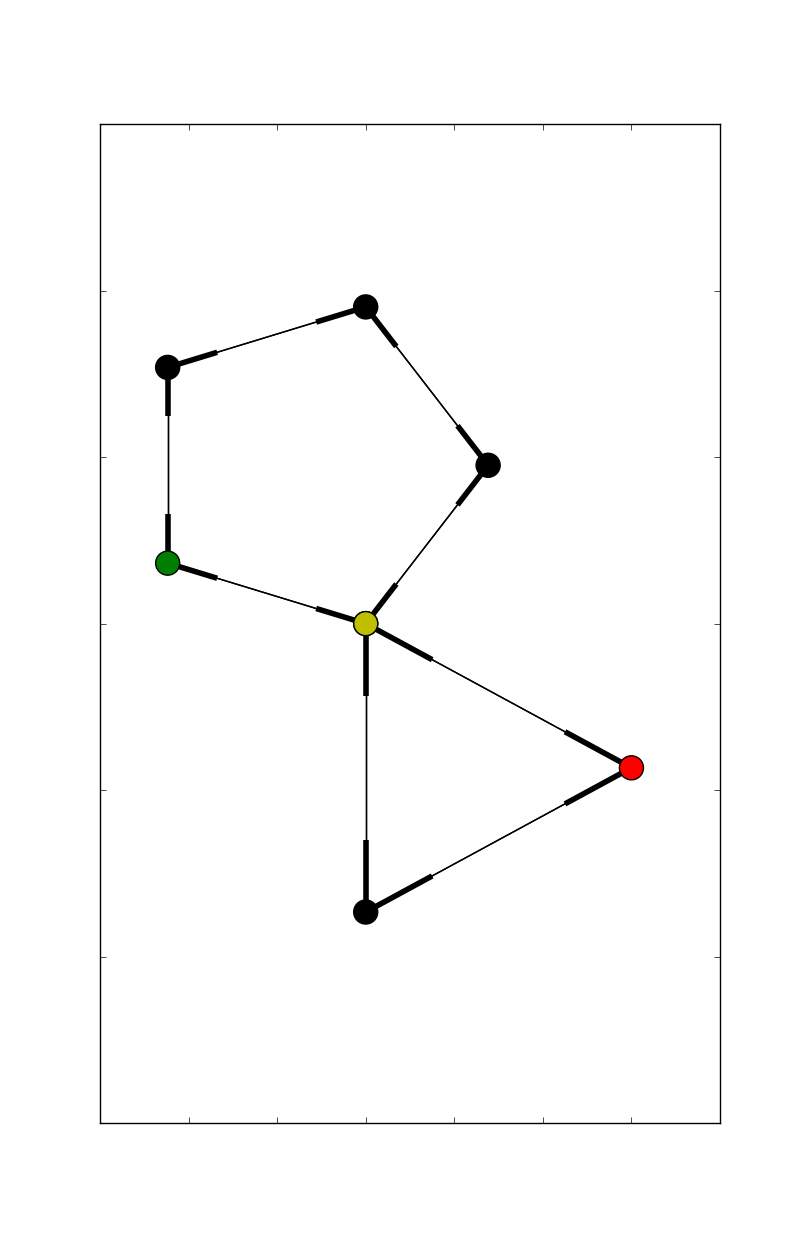
\includegraphics[height=0.5\textheight]{imgs/pattern_joined}
  \caption{Graph topology used to reproduce a more complex pattern: Two cicular topologies joined at the yellow node. The green and yellow nodes will have a phase shift of $\frac{2\pi}{5}$, the yellow and red nodes will have a phase shift of $\frac{2\pi}{3}$. This gives a total phase shift of $\frac{2\pi}{5} + \frac{2\pi}{5} = \frac{8 {\cdot} 2 \pi}{15}$. }
  \label{fig:pattern_joined}
\end{figure}

There is however a slight problem still: We have no guarantee that the total phase shift is indeed the sum of phase shifts in the individual circles. Since the phase shifts could propagnate in different directions the total phase shift could actually be the difference. We can work around this however by choosing the correct initial values for the oscilators -- both states are equally stable. 

Finally we can note that it is possible to further expand these patterns. Instead of just two circles, we can take more circles to produce offsets of the form

\[
  \sum_{i}{\frac{q_i {\cdot} 2 \pi}{p_i}}
\]

with $p_i$ prime and $q_i \in \mathbb{N}$. In fact if we take into account that we are operating modulo $2 \Pi$ we can even take $q_i \in \mathbb{Z}$. 
Now given any phase shift $\frac{p {\cdot} 2 \pi}{q}$ we can obviously use the prime factors as denominators $p_i$ and write it in this form. We can then use the procedure described above to create a topology that can produce the given phase shift. 

If we have more than two oscilators in a pattern that we want to construct, we can also continue this procedure. We can just join more circles to the node we want to define a phase shift relative to. 
	\newpage
	
	% Section 5
	\section{Conclusion}
	\ednote{Tom + Alee: Write this}
	
	% TODO: Proper references ? 
\end{document}